% Supporting Information — integrated polypharmacology and RRS study
\documentclass[journal=jcisd8,manuscript=suppinfo]{achemso}
\usepackage[T1]{fontenc}
\usepackage[utf8]{inputenc}
\usepackage{lmodern}
\usepackage{amsmath,amssymb}
\usepackage[detect-all=true,group-minimum-digits=4]{siunitx}
\DeclareSIUnit\angstrom{\text{\AA}}
\DeclareSIUnit\calorie{cal}
\usepackage{booktabs,tabularx,array,longtable}
\usepackage{xr}
\usepackage[colorlinks=true,linkcolor=blue,citecolor=blue,urlcolor=blue]{hyperref}
\usepackage[noabbrev,capitalize]{cleveref}
\externaldocument[M-]{P1_V6_Integrated_Polypharmacology_RRS}
\graphicspath{{Graphics/}}
\author{Myke Vital Sao Temgoua}
\author{Jean-Pierre Tchapet Njafa}
\author{Penabei Samafou}
\author{Wilfred Fon Mbacham}
\author{Serge Guy Nana Engo}
\title{Supporting Information: From African-Natural-Product Chemical Space to Resistance-Resilience Hypotheses}
\begin{document}

\noindent This supplement contains the numerical material needed to reproduce the integrated computational analysis. It is organized by evidence layer: chemical space, target-anchored docking, RRS, and exploratory cross-metric analysis. The four-target matrix is reported target by target; no cross-target mean is used because the Vina score is not calibrated across unlike receptor pockets.

\section*{S1. Cohort and evidence boundaries}
The integrated analysis uses the 17-member P2 Set-C polypharmacology-oriented cohort. The docking calculations follow AutoDock Vina conventions \cite{Trott2009,Eberhardt2021}. The MPO top-20 and the parent-study MD top-20 are distinct sets. The parent-study MD systems 201, 438, the 164-labelled PfClpR cohort, and 214 are not MD validation of Set C. The target panel contains four wild-type docking profiles, whereas RRS is calculated from the separate `docking\_mutants.csv` WT/mutant panel and is available only for PfDHFR and PfCRT mutant panels.

\section*{S2. Target-anchored docking matrix}
\begin{table}[h]
\centering
\caption{Target-anchored Vina estimates for the locked 17-member cohort. Values are in \si{\kilo\calorie\per\mole}; they are not experimental free energies.}
\label{tab:vina}
\small
\begin{tabular}{@{}lrrrr@{}}
\toprule
Candidate & PfDHFR & PfCRT & PfClpP & PfATP4 \\
\midrule
PP-01 & \num{-5.947} & \num{-6.483} & \num{-5.467} & \num{-6.361} \\
PP-02 & \num{-5.562} & \num{-6.124} & \num{-5.907} & \num{-6.591} \\
PP-03 & \num{-6.089} & \num{-6.633} & \num{-6.358} & \num{-7.311} \\
PP-04 & \num{-5.493} & \num{-5.329} & \num{-5.386} & \num{-6.086} \\
PP-05 & \num{-6.285} & \num{-6.412} & \num{-6.466} & \num{-6.378} \\
PP-06 & \num{-6.267} & \num{-7.907} & \num{-7.031} & \num{-7.285} \\
PP-07 & \num{-6.226} & \num{-6.633} & \num{-6.226} & \num{-5.775} \\
PP-08 & \num{-4.935} & \num{-5.213} & \num{-5.052} & \num{-5.494} \\
PP-09 & \num{-5.693} & \num{-6.871} & \num{-5.613} & \num{-6.078} \\
PP-10 & \num{-6.346} & \num{-6.395} & \num{-6.016} & \num{-6.670} \\
PP-11 & \num{-6.179} & \num{-6.376} & \num{-6.583} & \num{-6.724} \\
PP-12 & \num{-5.248} & \num{-6.357} & \num{-5.386} & \num{-4.635} \\
PP-13 & \num{-5.921} & \num{-5.685} & \num{-6.454} & \num{-7.565} \\
PP-14 & \num{-4.863} & \num{-5.328} & \num{-5.047} & \num{-5.460} \\
PP-15 & \num{-6.045} & \num{-6.084} & \num{-6.366} & \num{-7.016} \\
PP-16 & \num{-5.469} & \num{-6.202} & \num{-6.203} & \num{-6.451} \\
PP-17 & \num{-5.266} & \num{-5.116} & \num{-5.342} & \num{-5.360} \\
\bottomrule
\end{tabular}
\end{table}

\begin{figure}[h]
\centering
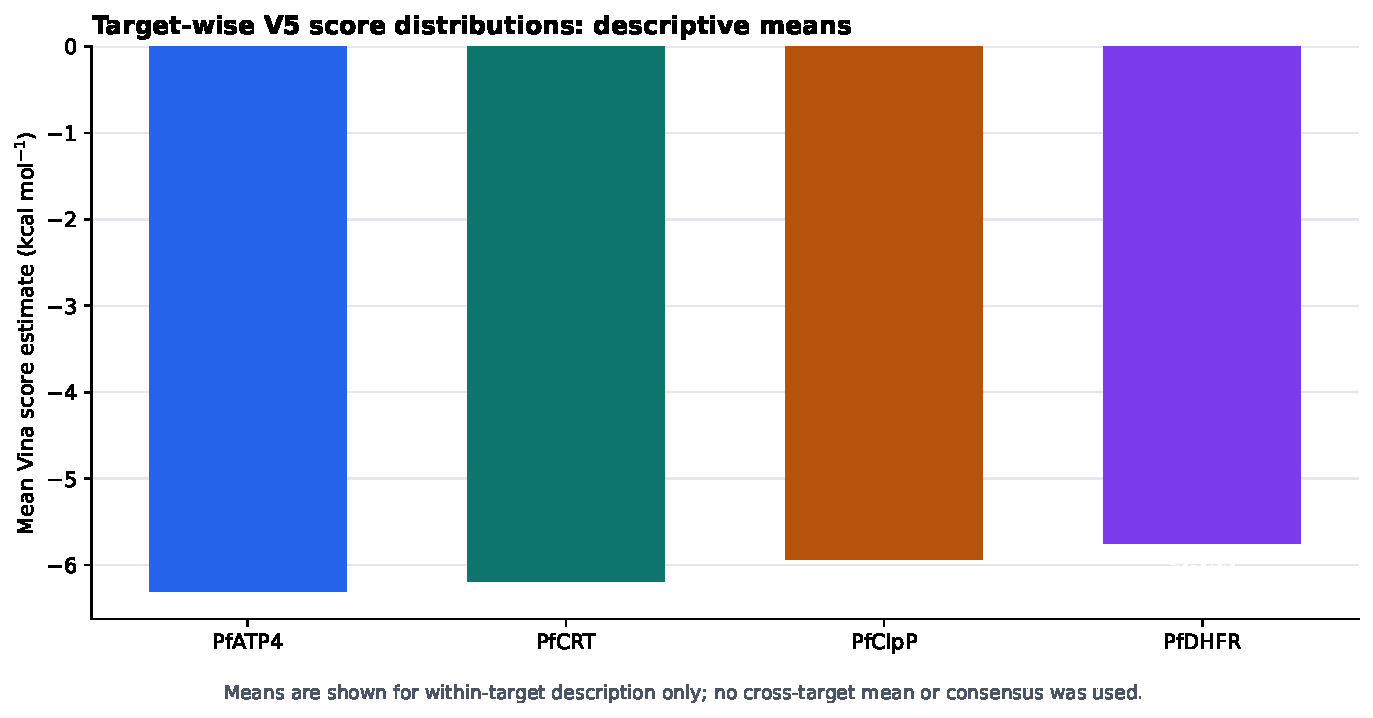
\includegraphics[width=0.95\textwidth]{p1_v6_targetwise_profile_summary.pdf}
\caption{Descriptive target-wise means from the raw docking panel. Means are shown only within target; no cross-target arithmetic mean or consensus score was used. These summaries are computational scoring-function outputs, not experimental affinity measurements.}
\label{fig:targetwise_summary}
\end{figure}

\section*{S3. RRS definition and class summary}
For candidate $i$, mutation $m$, and target $t$:
\[
\mathrm{RRS}_{i,m,t}=100|S_{\mathrm{Vina},i,m,t}|/|S_{\mathrm{Vina},i,WT,t}|.
\]
Here $S_{\mathrm{Vina}}$ denotes an AutoDock Vina scoring-function output, not an experimental free energy. RRS eligibility is determined from the separate `docking\_mutants.csv` WT/mutant panel, not from the four-target V5 wild-type matrix. Only genuine wild-type binders with $|S_{\mathrm{Vina},i,WT,t}|\geq\qty{5}{\kilo\calorie\per\mole}$ contributed. The 17-candidate class counts were A*: \num{6}, B: \num{5}, C: \num{5}, and D: \num{1}. The observed RRS range was \numrange{68.2}{111.7}. The complete machine-readable values are in \texttt{Project2\_Polypharmacology\_MD\_ValidationV2607/results/c\_rrs\_classification.csv}.

\begin{table}[h]
\centering
\caption{RRS class definitions used in the integrated analysis.}
\label{tab:rrs_classes}
\begin{tabular}{@{}lll@{}}
\toprule
Class & Operational definition & Number \\
\midrule
A* & maximum absolute eligible WT score $\geq\qty{7}{\kilo\calorie\per\mole}$ and all available RRS values $\geq\qty{80}{\percent}$ & 6 \\
A & All available RRS values $\geq\qty{80}{\percent}$, without the A* wild-type criterion & 0 \\
B & All available RRS values $\geq\qty{70}{\percent}$, but not all $\geq\qty{80}{\percent}$ & 5 \\
C & At least one RRS value $\geq\qty{80}{\percent}$, with the complete-panel criteria for A/A* or B not met & 5 \\
D & No available RRS value $\geq\qty{80}{\percent}$ & 1 \\
\bottomrule
\end{tabular}
\end{table}

\section*{S4. Exploratory cross-metric analysis}
\begin{table}[h]
\centering
\caption{Spearman correlations on the 17-member cohort. Bonferroni-adjusted threshold: $\alpha=\num{0.017}$ for the three hypothesis-oriented comparisons.}
\label{tab:crossmetric}
\begin{tabular}{@{}lrrl@{}}
\toprule
Pair & $\rho$ & $p$ & Interpretation \\
\midrule
PNS--RRS & \num{-0.559} & \num{0.020} & Nominal trend; not Bonferroni-significant \\
ACSI--RRS & \num{-0.132} & \num{0.613} & Not significant \\
RRS--wild-type Vina score & \num{-0.433} & \num{0.082} & Not significant \\
PNS--wild-type Vina score & \num{0.389} & \num{0.123} & Descriptive/mechanical comparison \\
\bottomrule
\end{tabular}
\end{table}

\section*{S5. Target evidence classes and limitations}
PfDHFR uses a catalytic-site ligand anchor; PfClpP uses a catalytic triad; PfCRT uses a membrane-associated Y01 cavity proxy; and PfATP4 uses conserved P-type ATPase machinery without a co-crystallized inhibitor. Consequently, all four-target profiles are exploratory and are not equivalent evidence of biological target engagement. No RRS values are reported for PfClpP or PfATP4.

\section*{S6. Reproducibility and availability}
The integrated candidate manifest, raw docking table, P2 RRS table, cross-metric matrix, scripts, receptor files, ligand files, and provenance records are available in the repository at \url{https://github.com/NanaEngo/Malaria_codesV2}. The figures and derived tables in this supplement are reproducible computational outputs; automated integrity checks document their derivation but do not substitute for independent structural or experimental validation.

\bibliography{Sao_Chim_Space}
\end{document}
